
    \section{How do we know when we succeeded?}
    
        \subsection{Making a toy resonator from Nb$_3$Sn that's better than Cu i.e. $Q > 10^6$}
        
        The run time for ADMX's extended frequency range (EFR) search, could be cut in half from 4 years to 2 if prototype superconducting cavities can be scaled up and we can achieve a quality factor of $10^6$ in 9T magnetic field. 
        
        \subsection{Correlate recipes with quality factor: Process $\to$ structure \& composition $\to$ $Q$  }

        Though the final quality factor achieved was not as high as we would have liked, we created a prototype with clear steps to improve the quality factor of these cavities. We will study these cavities to gain insights into the physics of dissipation in the cavity due to surface roughness, Sn concentration, thickness uniformity, and impurities in the bulk and grain boundaries. This would allow us to link the quality factor measured with the microstructure of different recipes. After we have tested the RF properties, we will cut up the cavity to analyze the microstructure.

        One question of interest is how the film morphology on surfaces not perpendicular to the source looks like. One way to do this is to use in-situ coupon analysis. One fabricated cavity with holes for coupon samples and one without. These samples sit flush with the inner surface of the cavity during all fabrication steps. Once the Nb$_3$Sn film has been made, one cavity goes in for RF testing, and the other cavity's coupon samples are analyzed. A similar in-situ coupon analysis was done by \citeauthor{Viklund:2023nlq} \cite{Viklund:2023nlq} to analyze the roughness of Nb$_3$Sn after barrel polishing.
        
        \begin{figure}
           \centering
            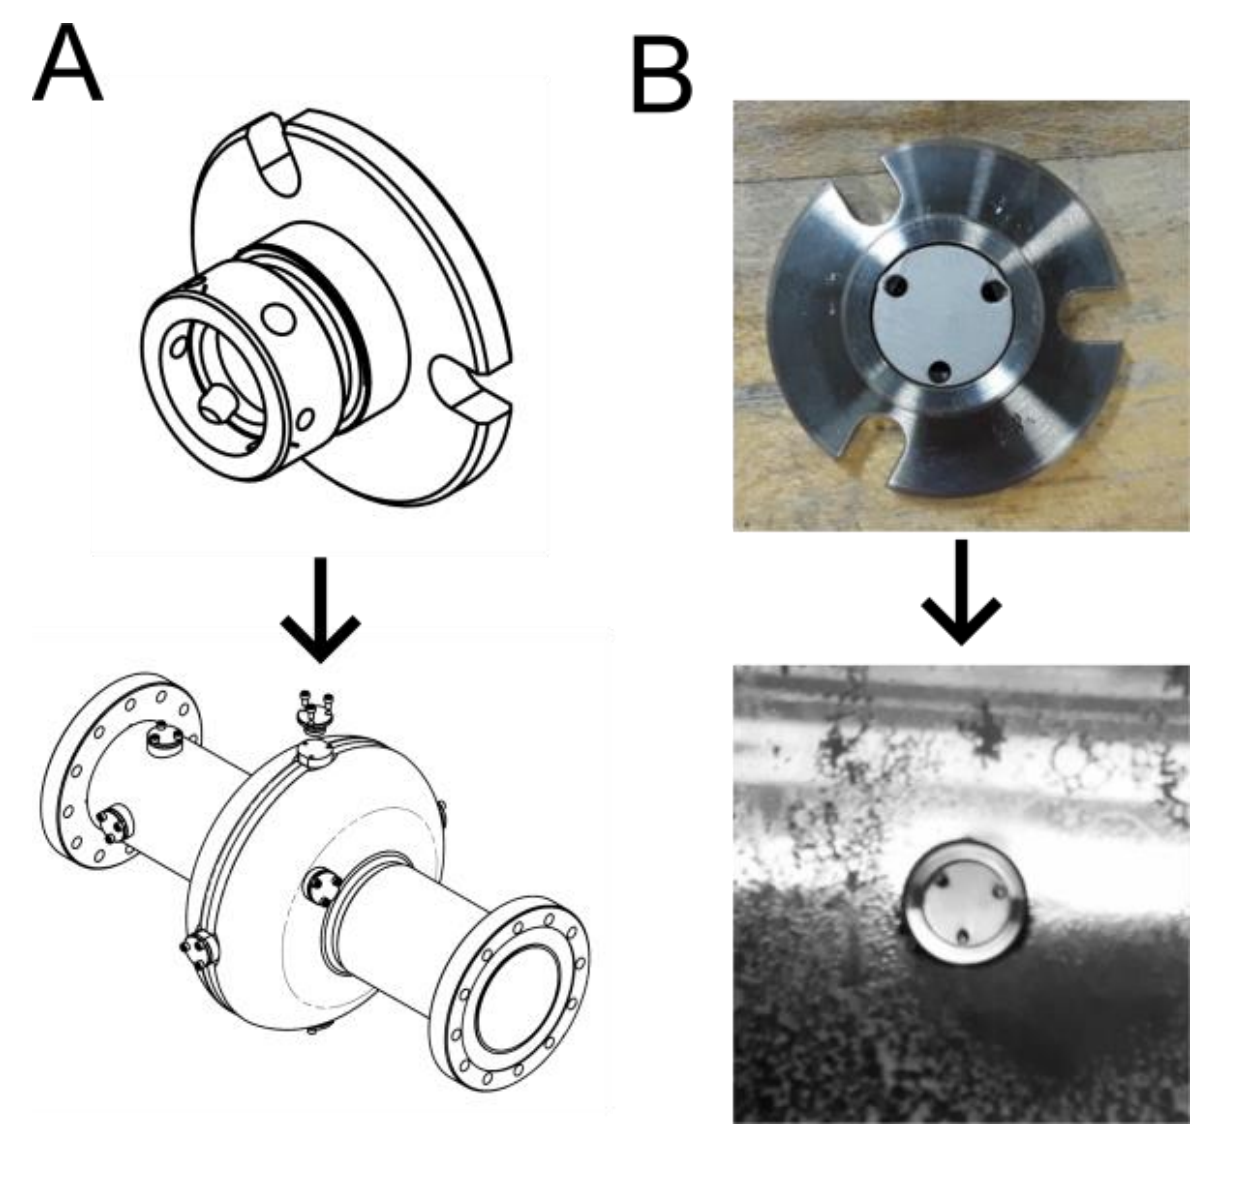
\includegraphics[width=.5\textwidth]{images/Future/ViklundCoupon.png}
            \caption{Coupon sample used to measure the surface roughness at different locations inside a Nb$_3$Sn cavity. \cite{Viklund:2023nlq}}
            \label{fig:ViklundCoupon}
        \end{figure}

        The first RF Nb$_3$Sn cavities will use the recipes shown in the above subsections:  Cu-Sn on Cu/Ta/Nb or Cu/Nb, with a post-reaction and an etch, and Nb on Cu/Ta/Cu-Sn, with a hot-bronze and post-reaction. We can explore other routes if needed.

        
    \section{Optimize the routes with the best properties, further.}
    
        \subsection{ Cu substrate with Cu-Sn film on Ta/Nb or Nb with post-reaction and etch }
        
        Using a Nb-Cu-Sn route, there are several possible routes for fabricating Nb$_3$Sn on Cu. The films with the best microstructural uniformity possess a Cu-Sn film as the final layer, as seen in Figure \ref{fig:BronzeOnNb}. The Cu-Sn film contained void space due to the high mobility Sn atoms. When Nb is deposited onto a Cu-Sn film, the resulting Nb$_3$Sn follows the rough heterogeneous Cu-Sn film. This resulting uneven Nb$_3$Sn film will perform worse in RF $Q$ testing. This method required an APS etching afterward to remove the Cu-Sn surface layer. 
            
        \begin{figure}[ht!]
            \centering
            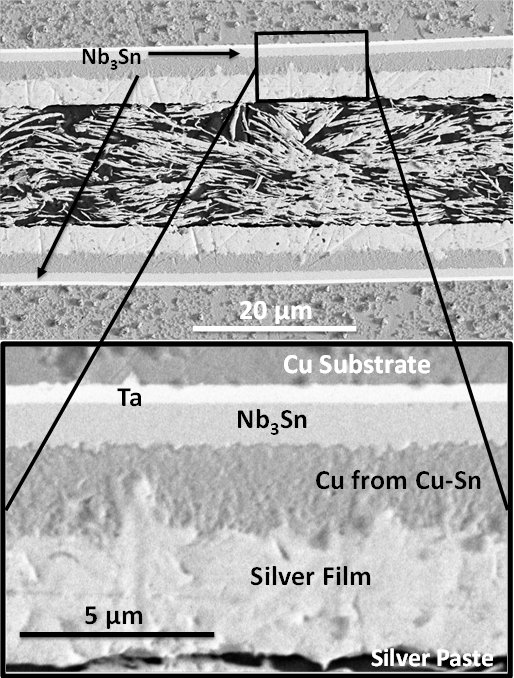
\includegraphics[width=.5\textwidth]{images/Cu/BronzeOnNb/BronzeOnNb.png}
            \caption[SEM Image of two Nb$\mathrm{_{3}}$Sn film's sandwiched together.]{SEM Image of two Nb$\mathrm{_{3}}$Sn film's sandwiched together. This film was synthesized with Nb/Bronze on Ta rather than the usual Bronze/Nb on Ta. This sample was made using the post-reaction recipe.} %Do we have EDS for these samples and Tc, this looks very good!
            \label{fig:BronzeOnNb}
        \end{figure}
          
    
        \subsection{Cu substrate with Nb film on Cu-Sn layer using hot-bronze and post-reaction}
        
        The Nb$_3$Sn films with the best critical temperature were those where Nb was deposited at high temperature $\sim$ 700 $^{\circ}$C onto Cu/Ta/Cu-Sn. These samples immediately reacted with the hot Sn in the Cu-Sn film and post-reacted to increase the $T_c$ further. These films did not require an etch afterward if the Nb$_3$Sn is the terminal surface layer. A scanning electron microscope (SEM) and electron diffraction spectroscopy (EDS) cross-section portray the microstructure and concentration of elements, as shown in Figure \ref{fig:WenuraEDS} of this film.
        
        \begin{figure}
            \centering
            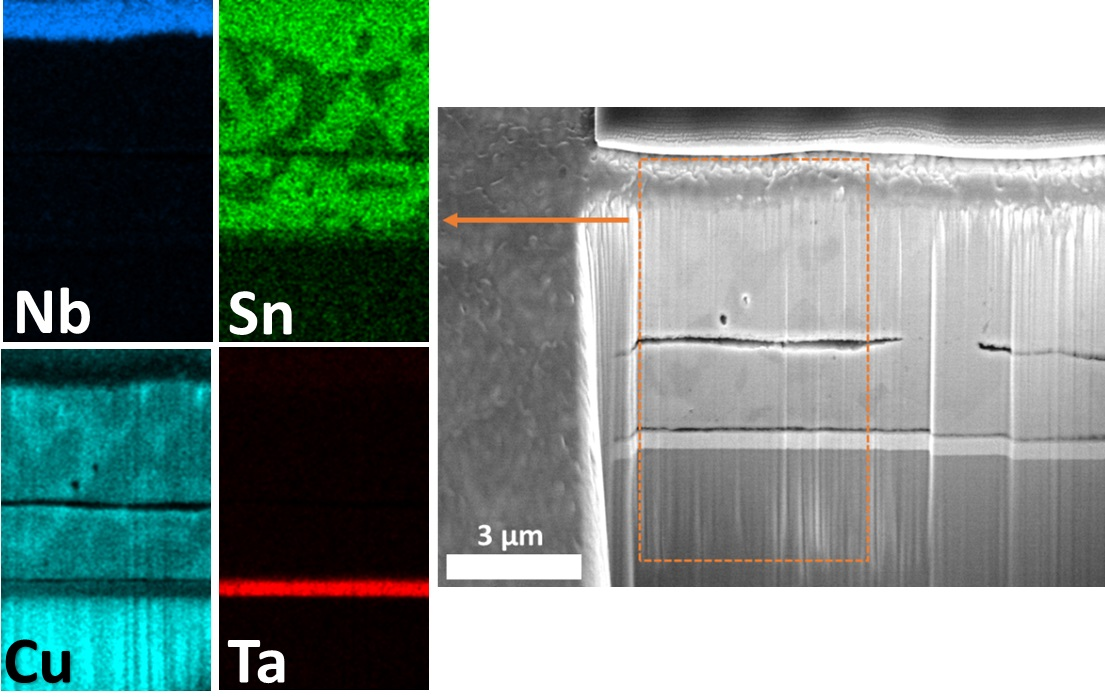
\includegraphics[width=\textwidth]{images/Cu/CuSnThickness/wenura EDS SEM.jpg}
            \caption{A Cu substrate with a 400nm Nb$\mathrm{_{3}}$Sn film on 5µm of Cu - 33\% wt Sn and a 500nm thick Ta diffusion barrier. Typical void formation in many bronze processes is found in our Cu-Sn layer. This void space can relieve strain on the Nb$\mathrm{_{3}}$Sn, leading to higher Tc.}
            \label{fig:WenuraEDS}
        \end{figure}
          

        %\subsection{Other Routes, but only as backups}




    \section{Setting up an RF measurement system relevant to ADMX}

        \subsection{Prepare the Cu cavity}


        Two Bulk oxygen free electrolytic high conductivity (OFHC) Cu with dimensions of (7 x 3 x 1.5 cm) will be purchased as the starting material for the two half-shells. A simulated CAD geometry of the two half shells with two input couplers, a thermocouple on top and bottom, and a mount from the top will be made, and it must fit within the dimensions of the magnet shown in Figure \ref{fig:ULFMagnet}, and will be similar to the design in Figure \ref{fig:CADCavityProto}. We will use the CAD design and machine our geometry from the bulk blocks. We will polish the interface edge, so the two pieces will fit snugley together, and electropolish the inner resonating surface to decrease surface roughness. Surface roughness will reduce the quality factor of the cavity. We will bolt the two half-shells together, and attach two solder connectors to the top cavity. This connector will allow us to attach two co-axial cables, that give us control to measure the frequency and quality factor of the cavity. 
        
        \begin{enumerate}
            \item Purchase two Bulk Cu oxygen-free high conductivity (OFHC) (7 x 3 x 1.5 cm) blocks
            \item Prepare CAD design for resonator from two half shells
            \item Machine the resonator out of bulk pieces using CAD design 
           \item Polish interface edges
            \item Electropolish the resonating surface
            \item Bolt together two half-shells
            \item Attach the solder connector to the top cavity end-cap
        \end{enumerate}



        \begin{figure}
            \centering
            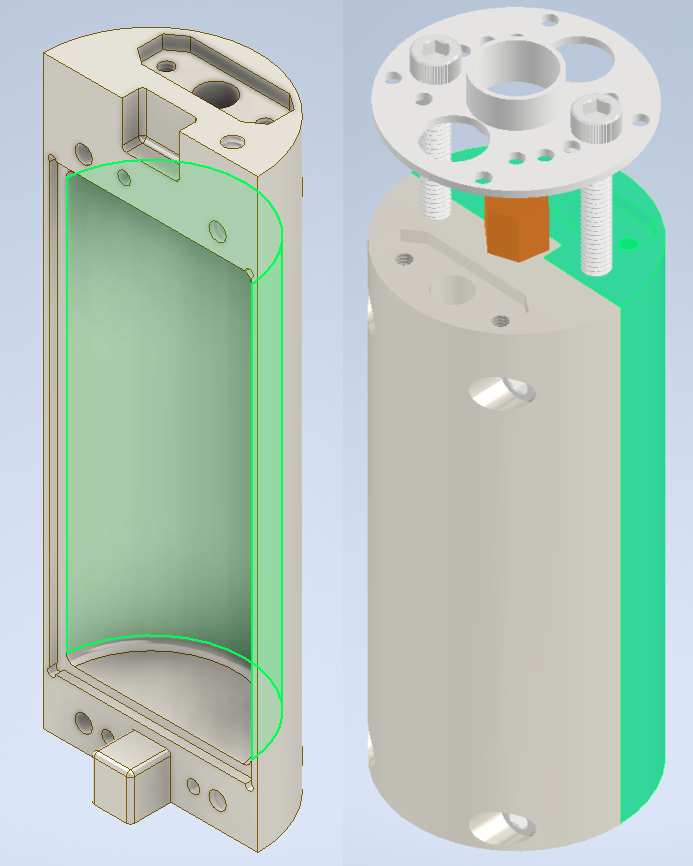
\includegraphics[width=.5\textwidth]{images/AndreCavity/CADCavityProto.png}
            \caption{This design is for a resonator that fits into a magnet, where the two holes on the top are for RF in and out. The top piece is mounted onto a probe and lowered into the magnet center. There is an orange thermocouple at the top of the resonator. The Nb$_3$Sn film will be coated on the highlighted green surface in the left image. \cite{Braine:2022qal}}
            \label{fig:CADCavityProto}
        \end{figure}
          
            
        \subsection{Test the Cu cavity at room temperature and 0 magnetic field}

        We will connect the connect one end of the co-axial cables to the top plate solder leads and the other end of the cable to a vector network analyzer (VNA) with a range of 1-20 GHz. We can start to measure the cavity mode, and cut away the RF input cable until the resonator is as weakly coupled to the cavity as possible, but still has a reflection dip. We can record the TM$_{010}$, TM$_{011}$, TM$_{012}$ modes. With this data we can analyze which surface contributes to which quality factor given as the ratio of cavity modes.
    
            
        \subsection{Test Cu cavity at 4.2 K and 9 T}

        We would like to get quality factor measurements in magnetic field and at low temperature so we can compare the results from Cu to the superconducting cavity. We will mount the Cu cavity measured in the previous step, onto a probe that can be lowered into a magnet. We will lower this probe with the Cu cavity on the end, into a 145 mm bore, 9 T magnet, shown in Figure \ref{fig:ULFMagnet}, and cool the magnet. We will allow the cavity to thermalize for $\approx$ 10 min, and record the frequency peaks at 0 field. We will ramp the magnet at $\Delta$.1 T from 0 T$\rightarrow$1 T and at $\Delta$1 T from 1 T$\rightarrow$9 T held for $\approx$ 1 min at each step to measure $Q$. The standard Cu cavity should reach $Q \sim 10^5$ 4.2 K in 6 T background field. 
        
            %\begin{enumerate}[label=\alph*)]
            %    \item Design probe to support and attach to the cavity
            %    \item Machine the Probe
            %    \item Mount the Cavity onto the Probe
            %    \item Cool the magnet to 4.2 K
            %    \item Insert the probe into the magnet
            %    \item Allow cavity to thermalize $\approx$ 10 min
            %    \item Record peaks at 0 field
            %    \item Ramp magnet at $\Delta$.1 T from 0 T$\rightarrow$1 T and at $\Delta$1 T from 1 T$\rightarrow$9 T held for $\approx$ 1 min at each step to measure Q
                %\item Convert $Q$ to RS using Gn
            %\end{enumerate}

        
        %We can find surface resistance if we know the geometrical factor, which can 
        
        \begin{figure}
            \centering
            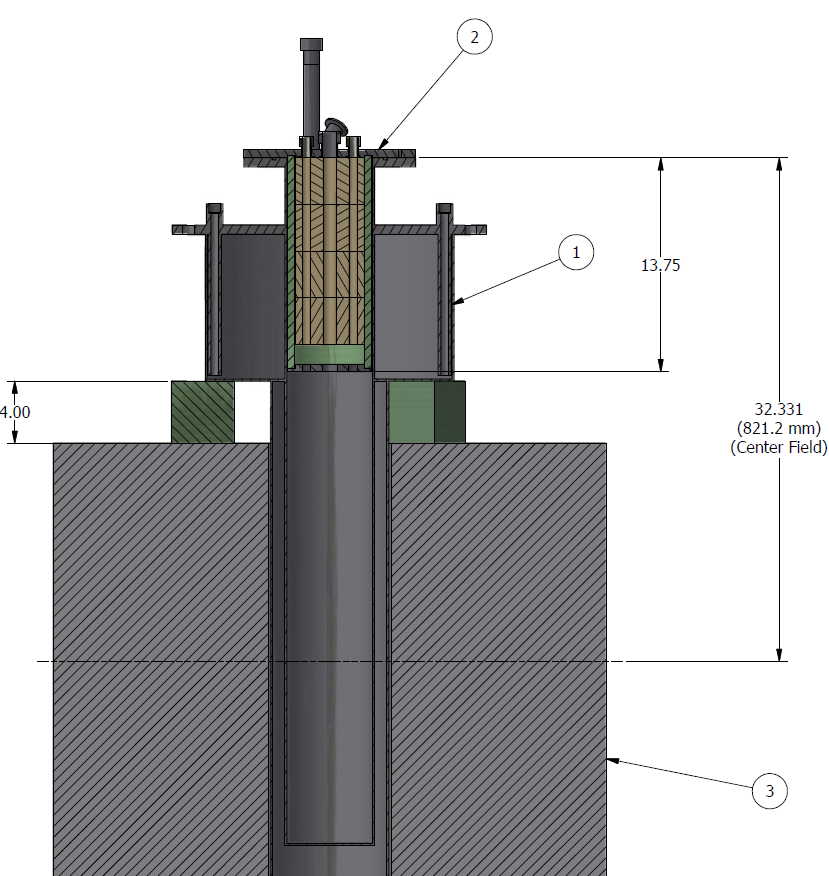
\includegraphics[width=.7\textwidth]{images/Future/ULFMagnet.png}
            \caption{A cryostat holding a 9 T, 145 mm bore magnet cooled to 4.2 K. The sample space can be filled with helium gas or helium liquid to cool down the sample. The sample is held from the probe, marked 2 on the diagram. The center field is where the resonator will be placed.}
            \label{fig:ULFMagnet}
        \end{figure}
          

    \section{Make and measure a Nb$_3$Sn cavity.}

        \subsection{Prepare for deposition}

        The substrate must be very clean before depositing the thin film, or the thin film will not adhere properly to the substrate. We will prepare another Cu cavity the same way we prepared the first Cu cavity. We will design a sample holder to constrain the Cu cavity above the evaporation and sputtering sources to allow for a line-of-sight deposition in the two chambers.
        
        %\begin{enumerate}[label=\alph*)]
        %    \item Follow subsection: Prepare the Cu cavity
        %    \item Fabricate the sample holder to hold half-shell for sputtering and evaporating
        %\end{enumerate}

            
        \subsection{Prepare Nb$_3$Sn (example recipe: Cu-Sn on Cu/Ta/Nb with a post-reaction)}

        We will one of the recipes prepared in early works. For example the Cu-Sn on Cu/Ta/Nb with a post-reaction recipe. This recipe starts with sputtering Ta then Nb on the Cu substrate. Then we place the cavity in the thermal evaporator and deposit a layer of Cu-Sn. We will bolt these two half-shells together, and heat treat in a high-vacuum tube furnace. After the Nb$_3$Sn reaction is completed we will etch the inner surface layer of Cu-Sn away with APS. $Q$ of the Nb$_3$Sn resonator will then be tested in the same way as was done with the Cu cavity.
        
        %\begin{enumerate}[label=\alph*)]
        %    \item Sputter the tantalum
        %    \item Sputter the niobium
        %    \item Evaporate the Cu-Sn
        %    \item Polish the interface between the half-shells
        %    \item Bolt together the two sections
        %    \item Heat Treat in a high-vacuum tube furnace
        %    \item Etch the surface layer of Cu-Sn with APS
        %    \item Follow subsection: Test Cu cavity at 4.2 K and 9 T, with Nb$_3$Sn cavity
        %\end{enumerate}

        One challenge with the preparation of this Nb$_3$Sn cavity is a non-uniform coating thickness because of deposition on complex geometry. The thermal evaporator source is 5 cm from the substrate, so the Cu-Sn film may not be as uniform in thickness unless special hardware accounts for the $\frac{1}{r^2}$ dependence of the vapor plume. Another option is using four shells instead of two or a hexagonal-shaped cavity if the uniformity of thickness is problematic. This will allow for a more planar substrate and an easier geometry to coat.
        
        Another challenge, is in the interface edge between cavities. These seams may not diffusion bond together if Nb is deposited onto this edge, so a mask is needed to cover the interface during deposition. Another option is to polish away any material that is deposited on the edge. The interface between shells must be clean if the goal is the binding of substrate pieces. If we require continuous superconductivity across the seam, it is prudent to post-react after the cavities are together, to allow the Nb-Sn reaction to convert to Nb$_3$Sn across the seam. The healing substrate experiment attempts to answer questions related to the healing of seams. 


      \section{Optimize the RF properties of the superconducting resonator.}

        The quality factor measurements yield a weighted average of all the losses in the cavity. This loss is related to:
        
        \begin{itemize}
            \item Surface roughness giving a higher apparent surface magnetic field
        \end{itemize}
        
        When a rough surface is in a magnetic field, the normal direction of the surface is in many different directions with respect to the static magnetic field. This causes the surface current in the superconductor to flow in different directions, which causes a magnetic field to be set up in many different directions. The surface can feel this newly induced magnetic field, which can be higher than the superconductor can take, so the Cooper pairs break down. If the roughness is lowered, these surface currents are generally in the same direction, and the apparent field felt by the material is closer to the actual field applied by the external magnet.
        
        \begin{itemize}
            \item Grain boundary impurities that the supercurrent has a hard time crossing
        \end{itemize}
        
        One of the key areas of investigation concerns the presence of impurities within the grain boundaries of Nb$_3$Sn films fabricated using the Nb-Sn-Cu route. In literature \cite{Tarantini:2021cum} Cu has been found at the grain boundaries despite its thermodynamic instability at the interface. A high-resolution study of our Nb$_3$Sn films' grain boundaries, specifically correlating quality factor with any observed impurities, would be valuable to the SRF community. When there are impurities in the Nb$_3$Sn lattice that replace the Nb or the Sn sites, the cooper pair density will decrease. Eventually given too many impurities, the material will not superconduct.
        
        \begin{itemize}
            \item Impurities in the bulk, low Sn $ < 25\%$ Nb$_3$Sn, or a highly strained lattice all reduce $T_c$, which lowers the amount of cooper pairs available to carry current
        \end{itemize}
        
        Nb$_3$Sn is not a line compound, which means there is a range of stable concentrations that this compound can be in a phase range of 18\% to 26\% at. Sn in the Nb$_3$Sn A15 matrix. The Nb$_3$Sn with the best critical temperature is when the Sn concentration is $\approx$ 25\% - 26\% at. Sn. 
        
        Cu substrates are particularly hard to fabricate Nb$_3$Sn onto, because the Sn will react with the Cu substrate, and the coefficient of thermal expansion (CTE) mismatch between Nb$_3$Sn and Cu is very large. This leads to low Sn Nb$_3$Sn and highly strained Nb$_3$Sn, respectively, which reduce the superconductor's critical temperature. For example, Nb$_3$Sn with the exact same composition on a Nb substrate vs a Cu substrate has the critical temperature depressed by 2 K by being confined to the Cu substrate. To control the loss of Sn to the Cu substrate, a diffusion barrier contains the Sn to the Cu-Sn film and the Nb film.
        
        \begin{itemize}
            \item A region less than three penetration depths thick $d > 3\lambda$ allowing supercurrent to travel in the Cu substrate
        \end{itemize}
        
        These films need a minimum thickness greater than 3 penetration depths ($3\lambda$), which is $\sim$ 300 nm for Nb$_3$Sn. The supercurrent falls off exponentially with penetration depth, so it is recommended that one has at least a $3\lambda$ thick film, to ensure the superconductor has sufficiently screened the supercurrent. This contains the current in the superconductor. If the superconductor is thinner than this value, the current can flow in the normal region which causes dissipation.
        
        \begin{itemize}
            \item The vortices are not strongly pinned and move around, causing dissipation
        \end{itemize}
        
        Our Nb$_3$Sn will be immersed in a strong magnetic field for the application of axion detection. This magnetic field will be strong enough to penetrate through the bulk of the superconductor. This comes in the form of quantized vortices, but the magnetic field is not strong enough to break down superconductivity altogether. The areas where the magnetic field penetrates the superconductor are regions that have normal electrons and no Cooper pairs. If this region does not move around the bulk of the sample, the super-current can navigate around this normal region and no dissipation will occur. But if these normal state regions do move they will cause normal ohmic dissipation due to the movement of normal electrons. These regions feel a Lorentz force from the external magnetic field, which can push them across the bulk of the sample. In some cases, these normal electron regions can be pinned on grain boundaries or impurities, which stops their movement and thereby reduces dissipation. 
  
        
 
